\documentclass[twoside,12pt,titlepage]{article}
\usepackage{setspace}
\usepackage[pdftex]{graphicx}
\usepackage[margin = 1in]{geometry}
\usepackage{enumitem}
\usepackage{amsmath}
\usepackage{siunitx}
\usepackage{fancyhdr}
\usepackage{chemmacros}
\setlength{\headheight}{15pt}

\newcommand{\machen}{Michael A. Chen}
\newcommand{\isotope}[2]{\ch{^{#1}#2}}
\pagestyle{fancy}
\lhead{\machen}
\chead{Thesis Proposal}
\rhead{\today}
\cfoot{\thepage}

\title{Studies of radioisotopes for use \\as tracers in groundwater systems}
\author{\machen}

\begin{document}
\maketitle
\thispagestyle{plain}

\begin{abstract}
Radioactive isotopes are naturally and anthropogenically generated compounds that have the potential to serve as tracers for key environmental processes. One compound of interest is radium, whose isotopes have found usage as tracers for groundwater flow into the ocean, and are a key contaminant in hydraulic fracturing operations. There are a number of key mechanisms, particularly sorption processes, that are not well understood for radium transport, and building understanding is crucial toward predicting groundwater flow and possible contamination of groundwater from hydraulic fracturing operations. Another example is \isotope{129}{I}, which is almost entirely sourced by anthropogenic nuclear activity. \isotope{129}{I} has the potential to serve as a powerful tracer for human nuclear activity, but these efforts are hampered by iodine having multiple oxidation states, and strong interactions with organic matter that result in the sorption and transformation of iodine. These interactions also suggest that iodine isotopes could be used as tracers for organoiodine in terrestrial environments. This work seeks to build a stronger understanding of these two compounds by a combination of batch sorption experiments, transport experiments in columns, and study in specific field sites in Pennsylvania and Hawaii to tease out the dominant mechanisms controlling these compounds' speciation and transport. This work will enable further usage of these radioactive isotopes as tracers for a wide range of environmental processes.
\end{abstract}

\section{Introduction}

In the past 100 years, radionuclides have become intimately tied with human society, serving as fuel sources, weapons, and tracers for both medical and environmental processes. Despite their ever increasing ubiquity, there is a strained relationship with these compounds, one often characterized by distrust and fear \cite{Hohenemser1977}. As one example, the 2011 Fukushima Dai-ichi Power Plant accident has driven some countries to abandon nuclear energy programs all together in attempt to avoid releases of nuclear material that could occur due to unforeseen circumstances. In parallel however, nuclear energy and medicine are still used globally \cite{Ramana2013}, and their waste products require careful treatment and disposal. One subject area requiring significant more understanding is the transport of these waste products in groundwater systems. As seen by the continuing work at the Savannah River, poor management of waste can lead to persistent contamination of groundwater \cite{Emerson2014}. Groundwater transport also plays an important role in the fate of contaminants at Fukushima, though many radioisotopes require further study \cite{Steinhauser2014}.
\par Among these radioisotopes, two elements stand out: Radium and Iodine. Radium has multiple isotopes that are naturally occurring in the environment, with a range of half-lives from a few weeks to thousands of years. While it has seen usage in the past in as a dubiously safe popular medicine, and as a luminescent compound, it currently sees little commercial usage \cite{WikiRadium}. Radium’s societal relevance comes not from its commercial usage, but from natural settings. Brines sourced from shales, which are sources for hydrocarbons used in hydraulic fracturing, or "fracking"', operations can contain up to \SI{0.7}{\nano Ci\per\liter} of Radium \cite{Barbot2013}, and must be carefully managed. Radium also has been identified as a key natural tracer for groundwater discharge into the ocean, where the natural background generation of radium isotopes is by thorium and uranium \cite{Moore2000}. Characterization of radium isotope transport properties similar to that of \isotope{137}{Cs} \cite{Steinhauser2014} is crucial toward using those isotopes in accurate transport based estimates of groundwater flow. 
\par The literature is peppered with a number of sources discussing the behavior of radium on solids. There were a number of studies measuring radium sorption on to various solids such as ferrihydrite, muscovite, and natural estuarine sediments, reporting a wide range of distribution coefficients \cite{Ames1983a,Ames1983b,Benes1984}. These studies formed a basis for understanding radium sorption behavior, but did not address the mechanisms of sorption or surface complexation. Later studies included other sediments \cite{Tachi2001} and radium saw the beginnings of its current usage as a groundwater tracer \cite{Moore1996}. Recent studies focusing on marine sediments compiled earlier work, finding huge variability in radium $K_d$ values, ranging from \SI{1.2}{\liter\per\kilo\gram} to \SI{38000}{\liter\per\kilo\gram}, with orders of magnitude variation occurring even with similar media and sorbent \cite{Beck2013}. There has been little study of radium in shale brines sourced by hydraulic fracturing outside of pure characterization \cite{Barbot2013,Rowan2011}. Thus there clear gaps in understanding radium behavior in fracking conditions as well as its surface complexation behavior.
\par Iodine is another element of interest with one naturally abundant, stable isotope, \isotope{127}{I}, and a few radioactive isotopes, \isotope{129}{I} and \isotope{131}{I}, whose major sources are anthropogenic nuclear activity \cite{He2013,Landis2012}. \isotope{127}{I} is a crucial micronutrient for human life that is found primarily in thyroid proteins \cite{Hu2009}. \isotope{129}{I} and \isotope{131}{I} are both radioactive isotopes that can be incorporated into the thyroid, leading to thyroid cancer, presenting a significant health risk during nuclear release accidents. Understanding its transport in soils and groundwater is thus crucial for both the maintenance and protection of human health. Additionally, the long half-life of \isotope{129}{I} and its low natural abundance suggest that it could be used as a tracer for nuclear material release \cite{He2013}. However, efforts to understand its transport are complicated by complex speciation behavior.
\par Iodine has a multitude of oxidation states, partitions significantly into organic matter, and can be volatile at environmental conditions, all of which affects its transport and speciation in groundwater systems. Fortunately, the only primary oxidation states for iodine in environmental systems are elemental iodine, \ch{I2}, iodide, \ch{I-}, and iodate, \ch{IO3-} \cite{Hou2009}. A figure illustrating these oxidation states can be seen in figure \ref{fig:IodineSpeciation}. Iodine also partitions into organic matter and there is evidence for both biotic and abiotic mechanisms for the incorporation of inorganic iodine into organic molecules \cite{Gilfedder2010, Yamaguchi2008}. Iodine cycling with respect to organic matter still has many unresolved questions, including the dominant mechanisms, and where those mechanisms come into play. Some of the iodine bearing organic compounds and elemental iodine are volatile, and can degas and escape from soils \cite{Hu2009}. Given the wide variety of forms iodine can take in a given system, significant effort has been made toward analytical tools to separate different forms of iodine. Common techniques take advantage of a chromatographic methods, such as high pressure liquid chromatography (HPLC) in combination with a ICP-MS to study iodine speciation \cite{Wuilloud2005}. Recent studies of transport behavior have leveraged these tools to study the behavior of the inorganic, aqueous iodine species and representative organoiodine compounds in specific media \cite{Hu2005}. Batch sorption experiments showed that iodine sorption is relatively weak to clay minerals, but stronger in the presence of reduced metal oxides and sulfides, and is almost entirely dominated by the presence of organic matter \cite{Assemi1994,Fuhrmann1998}. Similarly, there is not a clear understanding of even the basic kinetics and mechanisms of iodine incorporation into organic matter, nor is there strong understanding of the subsuquent transformation and release of those iodine species from organic matter, both biotically and abiotically \cite{Yamaguchi2008,Kaplan2014}. Careful characterization of these processes would enable iodine usage as a tracer for anthropogenic nuclear activity.

\begin{figure}
\centering
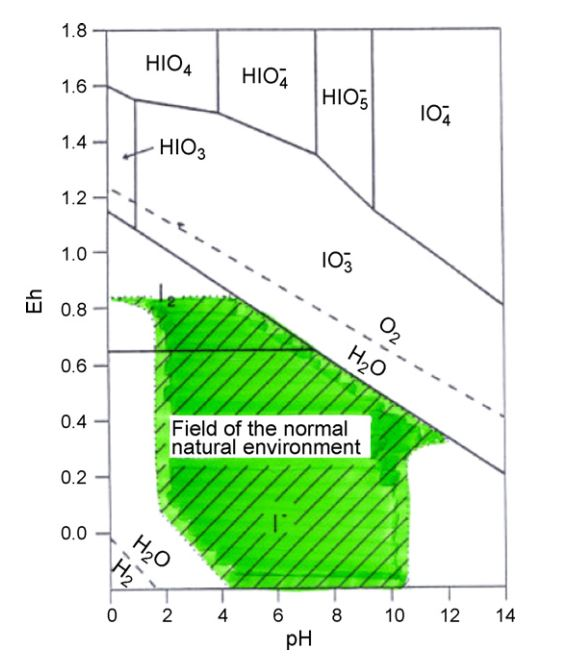
\includegraphics[width = 0.4\textwidth]{IodineSpeciation.png}
\caption{Eh-pH diagram for iodine in water at \SI{25}{\degreeCelsius}, with highlighting of common environmental conditions from \cite{Hou2009}.}
\label{fig:IodineSpeciation}
\end{figure}

\section{Objectives}

A common theme in studies of radium and iodine is developing or improving their functionality as environmental tracers in natural ground and surface waters. To this end, I broadly propose work that would serve to improve, augment, or enable their usage as tracer environmental tracers by developing specific understanding of the mechanisms controlling their transport and speciation.
\subsection{Radium}

\begin{enumerate}[label=\arabic*)]
	\item Radium transport in groundwater is dominated by a handful of minerals, and I expect it will be possible to build an accurate model of groundwater flow by accounting for these dominant minerals. I expect oxidized minerals, particularly iron and manganese oxides, to be prominent, if not the primary sorbing phases in environmental systems.
	\item I expect that in situ transformation from reduced minerals to oxidized minerals, or between oxidized mineral phases (as an example, ferrihydrite to goethite or hematite) will result in dynamically varying transport conditions for radium.
	\item I hypothesize that given radium's usage as a tracer in groundwater flow, and its elevated concentrations in produced water, it will be possible to trace surface water contamination resulting from improper storage of hydraulic fracturing wastes.
\end{enumerate}

\subsection{Iodine}

\begin{enumerate}[label = \arabic*)]
	\item Iodine speciation is a critical parameter controlling iodine transport, so I seek to study how organic matter and inorganic minerals control that speciation. I expect that in situ reduction and oxidation of minerals, notably iron and aluminum oxides that strongly sorb iodine species, can be paired with oxidation and reduction of iodine species to control iodine speciation.
	\item In spite of the complex iodine interactions with organic matter, it should be feasible to establish some basic parameters to establish constraints on iodine transport in the presence of organic matter. To this end, I would seek to characterize iodine sorption and transformation in organic matter, focusing on how organic matter composition, organic matter concentration, and system oxidation state affect those transport properties.

\end{enumerate}

\section{Proposed Research}

Given the large differences in the transport behavior of radium and iodine, work will be split along element specific sets of studies.

\subsection{Radium}

\subsubsection{Sorption Studies}
The first step in understanding radium transport behavior is to study basic Radium sorption behavior, using batch experiments with a single mineral in well controlled environments, using an appropriate isotope. Currently, I am using \isotope{226}{Ra}. Because of radium's $2+$ oxidation state and the few previous studies of radium sorption, I expect the major controlling element to be iron. As a result I plan to study, at minimum, the following minerals:

\begin{itemize}
	\item Ferrihydrite
	\item Pyrite
	\item Quartz
	\item Illite
\end{itemize}

\par Each of these minerals are representative of important mineral phases radium could encounter in a groundwater system. Ferrihydrite is a dominant environmental sorbent, often being the dominant sorbing phase in a given soil, even more so than other more thermodynamically stable iron oxides such as goethite or hematite \cite{Michel2007}. Pyrite is a representative reduced iron mineral, whose surface forms various iron oxides when exposed to oxygen, making it an ideal candidate for studies around the effects of mineral transformations on radium transport. Quartz and illite are silicate minerals that compose a significant fraction of shales used in hydraulic fracturing, and would be representative of common settings for radium \cite{Chermak2014}. Studies of sorption to these minerals will provide a basis for understanding the dominant phases that can sorb radium during groundwater transport.
\par There are previously established methods of making these minerals, or they can be purchased. Reduced minerals, like pyrite can form oxidized coatings \cite{Buckley1987}, so experiments with these minerals need to be performed anaerobically, while oxidized minerals can be used in normal lab conditions. Synthesized minerals can be standardized for their content by a combination of digestion and analysis with an inductively coupled plasma mass spectrometer (ICP-MS) or colormetric methods. Minerals that are made will also be taken to synchrotron facilities for structural analysis, using x-ray absorption near edge structure (XANES) and x-ray absorption fine structure (EXAFS) techniques \cite{Fendorf1999}. These methods can be used to confirm the mineral content and structures expected, as well as grant insight into sorptive behavior.
\par The second part of these batch experiments is controlling the solution that radium partitions into. Given the current lack of sorption data regarding radium, the media will be:

\begin{enumerate}[label = \roman*)]
	\item Pure water
	\item Artificial groundwater
	\item Artificial seawater
	\item Shale brine or equivalent high ionic strength solution
\end{enumerate}

Groundwater and seawater are common environmental media for subsurface settings, with some systems having both mixing. There are well established recipes for artificial groundwater and seawater such as those provided by ASTM \cite{ASTMSeawater2013}. It may be possible to use samples of groundwater or seawater from specific targeted sites for a more site specific characterization. Unfortunately, there isn't an established recipe for artificial brine, and access to natural shale brines may be limited by the companies running the natural gas extraction sites. These brines contain huge amounts of dissolved salts, an average of \SI{106390}{\milli\gram\per\liter} total dissolved solids (TDS), and exist at significantly different temperatures and pressures compared to seawater or groundwater. Thus I expect a major confounding factor in formulating a characteristic artificial brine will be preventing precipitation of various solids. Despite this, I expect to be able to create a representative, high ionic strength medium that is comparable to a shale brine, which can be used in these experiments. It may also be worthwhile to perform some of these experiments at elevated temperature, to better approximate the in-situ conditions in a shale.

\par In addition to variations in the media and mineral, I plan to perform a few types of batch sorption experiments. The first is a set of simple 24-hour sorption experiment, which I have already begun using \isotope{226}{Ra} and FHY in pH \num{3.5} water, whose preliminary results are shown in figure \ref{fig:RaFHYSorb}. The next experiment type is a time based sorption study, looking at the kinetics of the sorption process, as well as establishing an equilibration time for short term sorption processes. This experiment may need to run longer than 24 hours if I see variations in the sorptive behavior over longer times. The results of these experiments may help update the other possible experiments by giving a more accurate window of time for when equilibration occurs. The last set of experiments will be surface complexation studies, where the pH of the experiment is strictly controlled, which allows for a better understanding of the processes controlling radium sorption to these minerals.

\begin{figure}
	\centering
	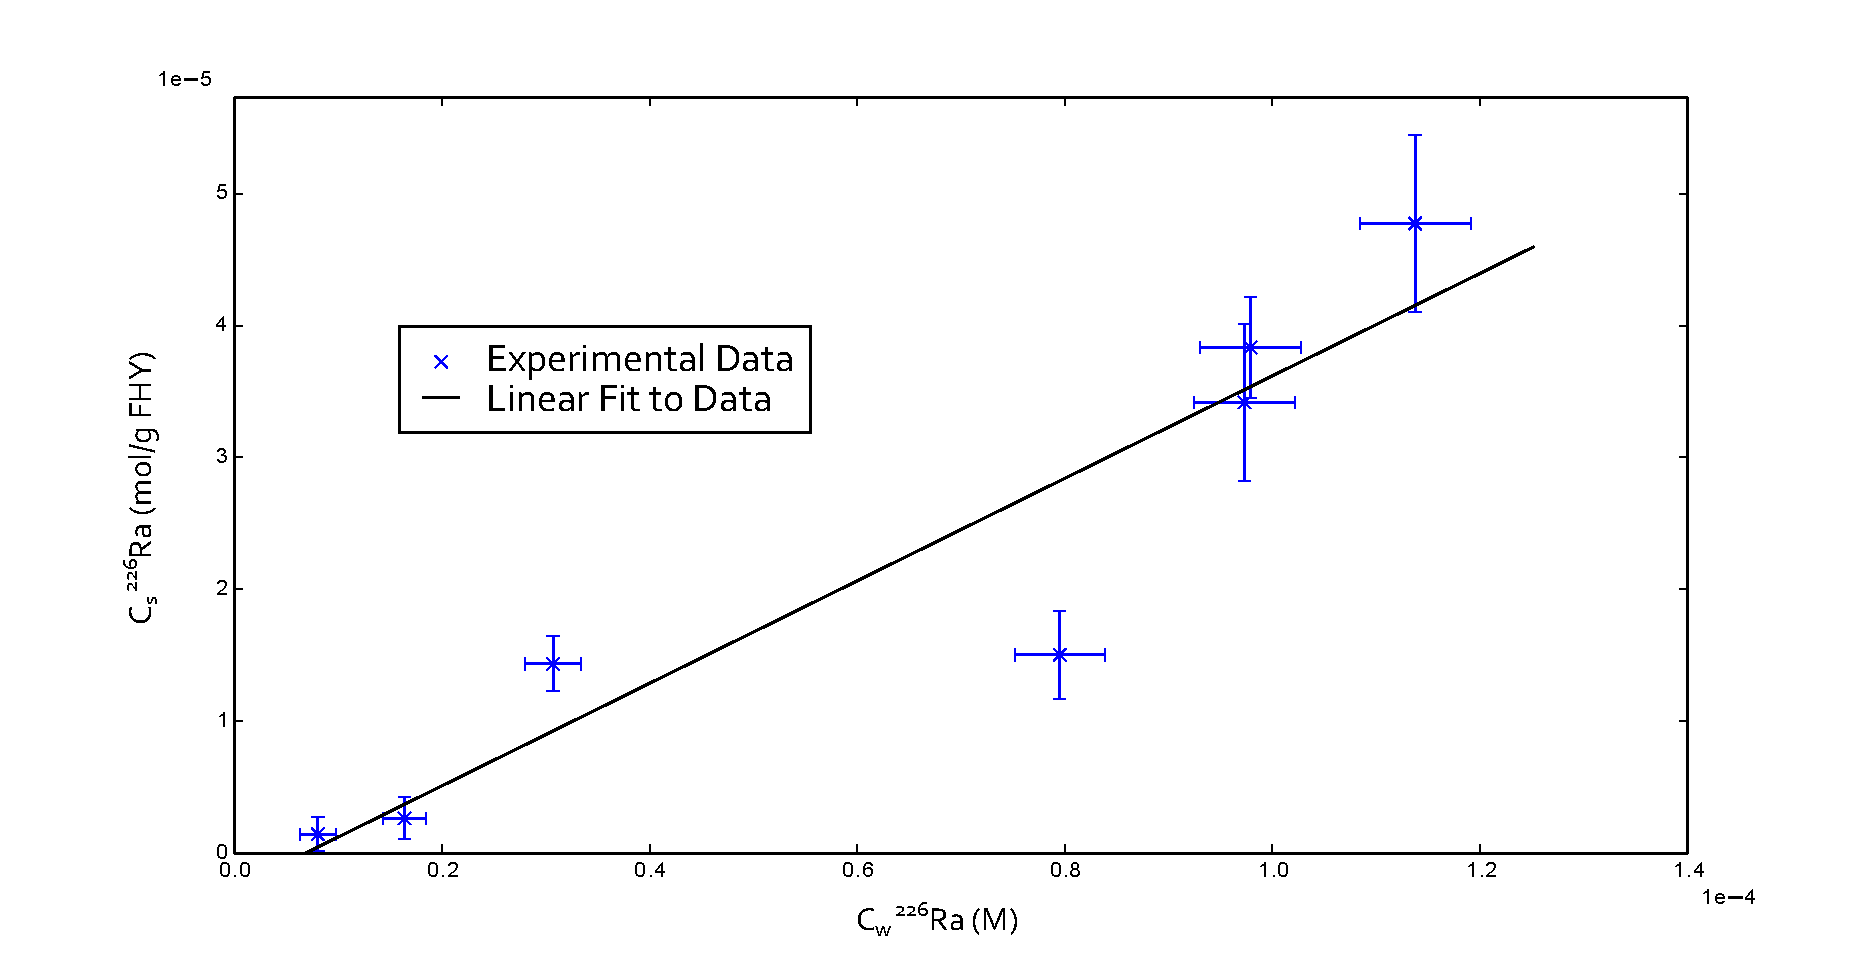
\includegraphics[width=0.8\textwidth]{AGU2014FHYRa.pdf}
	\caption{Figure showing preliminary sorption of \isotope{226}{Ra} to FHY in water at pH \num{3.5}. Error bars represent analytical uncertainty, and the linear fit is a simple polynomial fit using a NumPy polynomial fitting function. The fit gives a partition coefficient of \SI{0.39}{\liter\per\gram}.}
	\label{fig:RaFHYSorb}
\end{figure}

\par The data produced by these experiments provide the groundwork for modeling the sorption behavior of radium on these minerals. Fitting the equilibrated batch sorption experiments to a Langmuir or Freundlich type isotherm provides coefficients that can be used to predict solid-solution behavior in groundwater systems. This can be accomplished using a basic numerical tool such as the python package NumPy or more specialized software such as PHREEQC \cite{PHREEQC}. The time series experiments can be used to establish a foundational sense of the kinetics of radium sorption, examining how quickly equilibration can be reached. Lastly, the results of the pH controlled experiments can be fitted to build a surface complexation model that builds a picture of radium behavior on the surface of the various minerals, which can be accomplished with transport modeling software like PHREEQC or specialized tools \cite{Dixit2003}. This behavior can then be examined in further detail at synchrotron facilities by using XAFS and XANES methods on minerals with sorbed radium. This suite of models and fits will build a more complete picture of radium surface behavior, as well as help establish what minerals are dominant in controlling radium transport.

\subsubsection{Transport Studies}
\label{sec:RaTransport}
Soils, sediments, and fractured rock are porous media, comprised of a multitude of pore domains where mass transfer can be dominated by both advective and diffusive flow. While batch experiments can provide information on sorptive processes in pore domains with immobile water, further experiments are required to understand how hydrologic flow can affect radium adsorpiton and partitioning with(in) different the different minerals comprising a given porous media. The general procedure involves packing columns of an inert porous media (such as quartz sand) with a known, well distributed quantity of a mineral of interest from the previous batch studies. Flow of some water, be it pure water or a brine, would be pushed through the column containing a known concentration of radium, and measurements of the effluent from the column would be analyzed for radium concentrations. Variations in the timing, initial condition, and the constituents of these columns can be controlled to analyze different phenomena.
\par Initial phenomena I would wish to study is importance of sorption on the transport of radium in these columns. To study this, I would perform a series of column experiments containing increasing amounts of a strongly sorbing mineral such as ferrihydrite. In one set of experiments, I would saturate the column with a solution containing no radium, and then flow a solution containing a known concentration of radium through the column. The effluent of the column would be sampled for radium until the effluent concentration reaches a steady state condition. After this, I would then flow a solution without radium through, again sampling the effluent and measuring for radium until some steady state is reached. These time based experiments would establish a number of radium transport properties in ideal conditions. These include typical breakthrough times, equilibration times, retardation factors, and the strength of radium retention. Variations of the mineral and solution composition, similar to that in the sorption experiments would further elucidate important factors in transport, including the evolution of iron and manganese minerals and their impact on radium retention. These experiments in ideal conditions would then give way to experiments in less ideal conditions, using more complicated media and solutions. For example, soil cores from relevant field sites, such as those near Fukushima, or other field sites such as the Algehenny forest, where field work is currently planned \ref{sec:RaField}.
\par These column experiments represent idealized flow conditions that can help determine important adsorption/desorption parameters relevant to radium transport, but do not reflect the full complexity of typical groundwater systems where flow is multidimensional, as well as spatially and temporally variable. Thus these idealized columns must be connected to groundwater models that are calibrated to these ideal cases, which can then be used to predict behavior in more realistic groundwater systems. To do this, important properties of the idealized column experiment, including porosity, permeability, flow rate, and radium concentrations, are combined with sorption parameters to produce concentration profiles over time for certain regions of the column. These profiles can then be compared to profiles generated using groundwater modeling software such as PHREEQC \cite{PHREEQC} or MIN3P \cite{MIN3P}. Once calibrated, these models can then be run for complex groundwater domains to predict transport behavior in more realistic settings, providing flow dependent adsorption/desorption parameters.
\par It is possible that a reduced mineral such as pyrite could see a transition from anoxic conditions to oxic ones by the introduction of \ch{O2} rich waters or, in the case of fracking, if chemical oxidants are added. As an example, pyrite reacts with oxygen to form iron oxides:

\begin{reaction*}
FeS2{\sld} + 3.5 H2O{\lqd} + 3.75 O2{\gas} -> Fe(OH)3{\sld} + 4 H+ + 2 SO4\mch[2]
\end{reaction*}

This reaction results in dynamically changing conditions for radium transport dependent on the redox environment, thus it is important to study how temporal changes in redox conditions can affect radium transport. This can be accomplished through a column experiment where I attempt to alter a mineral present in the column, like pyrite, with the introduction of an oxidizing agent, such as potassium permanganate. These experiments would be operated in a similar manner as the simpler column experiments, but would involve tracking both amounts of radium and the oxidizing agent. This would simulate the introduction of chemical oxidants to alter soil geochemistry. Another experiment in this vein would be to pack a column with pyrite prepared under anaerobic conditions, removing any oxic coatings before the experiment, then flowing a solution at equilibrium with ambient air through the column to see how the transport properties evolve over time. This would represent a possible natural setting where anoxic porous media come into contact with oxygenated water, say in an estuarine region. These columns will also be run using only the oxidizing agent (or oxic water)and an aliquot of the resulting porous media will be taken to a synchrotron facility for mineral analysis. These experiments could be modeled as well, though more effort would be applied to establishing if these transformations would be useful and feasible for controlling radium transport in field settings.

\subsubsection{Field Campaign}
\label{sec:RaField}
Given the heightened risks of radium contamination as a result of hydraulic fracturing work, it is important to gather data on whether or not hydraulic fracturing operations are causing contamination of local surface water. To this end, I would propose a field campaign in northwestern PA, at the Allegheny National Forest to collect data on water quality near fracturing wells. National forest regions are ideal for this work, as the potentially affected watersheds sit on open access land, yet have a plethora of unconventional gas development, as seen in figure \ref{fig:NationalForest}. It may be possible to access some of the older storage sites or wells, though it is uncertain at this point whether or not the companies managing those facilities will allow direct access to their facilities for sampling. The data collected from these campaigns can then be tied to groundwater models of these watersheds.

\begin{figure}
	\centering
	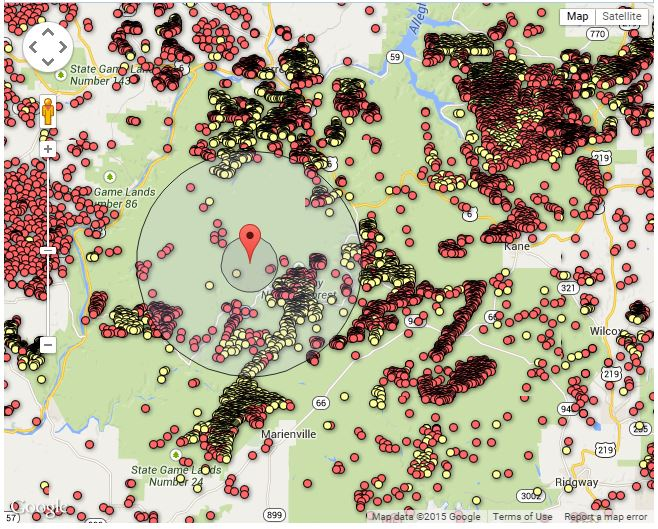
\includegraphics[width=0.5\textwidth]{AlghenneyForestFrackingWells.jpg}
	\caption{Figure depicting hydraulic fracturing wells drilled in the Alghenney National Forest. Red dots indicate wells where the amount of waste water discharge is unreported to the Pennsylvania Department of Environmental Protection (PADEP), while yellow dots indicate wells where the waste discharge amounts were reported \cite{NRDCFrackingMap}.}
	\label{fig:NationalForest}
\end{figure}

\par A major challenge in tracing geochemical impacts associated with unconventional gas development has been the selection of a tracer that can be exclusively linked to these activities. While radium is naturally sourced ubiquitously, brines associated with unconventional gas development contain elevated radium isotopes due to long equilibration times \cite{Barbot2013}. Thus it may be possible to attribute elevated radium isotope concentrations or differing radium isotope ratios to gas development. These isotopes may have migrated to local streams, sediments, or other components of the local water shed, so extensive surface water, sediment, and groundwater sampling will be necessary. These samples can then be analyzed for various radium isotopes using $\gamma$ or $\alpha$ spectrometry \cite{Elsinger1982,Bojanowski2005}. Due to the relatively low environmental background concentrations of radium, fairly precise analysis methods and large sample volumes will be necessary, which will be best accomplished by concentrating samples onto a resin. Barium, a compound with similar chemical behavior to radium, is another element commonly found in hydraulic fracturing wastes, and may also serve as a useful indicator for accidental waste release.

\subsection{Iodine}

In contrast to radium, there is already significant characterization of basic iodine sorption behavior, revealing the dominance of organic matter, followed by aluminum and iron oxides \cite{Kaplan2014}. Areas needing greater illumination center around iodine speciation and transformation, and how this more complicated behavior affects transport, and the focus of this work will be to tease apart parameters controlling those processes, with a focus on how those parameters focus on transport. This necessitates, given the diversity of organic matter and inorganic minerals found in environmental systems, a research focus on the iodine itself, rather than the media controlling its speciation. The general structure of this work is similar to the radium work, starting with batch experiments investigating speciation and transformation, followed by transport experiments, finally culminating in field work to understand environmental cycling of iodine in terrestrial systems. In this way, I will be able to develop a picture of the key parameters controlling iodine transport. This would then enable usage of \isotope{129}{I} as a tracer for nuclear activites, as well as enable its usage as a tracer for terrestrial cycling of iodine in organic matter.

\subsubsection{Sorption and transformation of iodine species at static conditions}
To probe the interactions of solid phases and iodine, I would first propose a series of batch time series experiments, where sorption parameters and iodine speciation is measured for up to 60 days. 60 days is the time scale over which some have seen complete incorporation of in organic iodine into organic matter \cite{Yamaguchi2008}. It will be instructive to examine both changes for an initial condition of only iodide vs one of only iodate. I expect to see changes in speciation over even shorter time periods, but would like to investigate the kinetics of this process. Additionally, I would like to see the impact of organic matter concentration, and organic matter type, comparing soluble humic acids to insoluble humin, as well as the effects of organic aging by comparing lignin, a common organic matter predecessor. There are two challenges in these experiments, the first is capturing iodine speciation in liquid samples. This can be done in a few ways, either through HPLC combined with ICP-MS as previously described \cite{Wuilloud2005} or by taking samples for analysis at the synchrotron using X-ray absorption near edge structure (XANES), which has been able to differentiate both inorganic species and organic ones \cite{Yamaguchi2008}. The second challenge in these experiments will be differentiating free solution iodine species and dissolved organic matter, which can be done through careful filtration processes. These experiments can establish a baseline set of static parameters for understanding iodine speciation and transformation during contact with organic matter.
\par The second set of experiments I would like to propose in this section involve purely inorganic iodine species and specific minerals, rather than organic matter. As discussed previously, minerals like pyrite and ferrihydrite can experience transformations in-situ by exposure to oxidizing or reducing agents. In this case, I would study how variations in oxidation state can affect both iodine speciation and sorption using pyrite and ferrihydrite. These minerals both sorb iodine species, and are demonstrated to be redox active, and would change in response to changing redox conditions. These would be done in batch experiments, without any flow condition, using appropriate atmospheric conditions (i.e. anoxic conditions for pyrite and iodate) as a time series with the introduction of a strong reductant or oxidant. Previous studies of iodine have shown that pyrite can reduce iodate to elemental iodine, which is a gaseous compound \cite{Kaplan2014}.  I would propose the use of illite as a control mineral because it lacks strong redox behavior, but is still able to sorb iodide \cite{Kaplan2014}. These experiments would provide a background of mineral impacts on iodine sorption during oxidative transformations, allowing for better understanding of iodine speciation in variable redox conditions commonly found in estuarine regions.

\subsubsection{Iodine speciation and partitioning with transport}
Building on the work of the previous section, the next step in understanding iodine speciation and transformation is to study these processes in conjunction with groundwater flow. Previous work has examined transport of iodine species using site specific sediments with high organic material, revealing a strong dependence on iodine concentration for retardation \cite{Zhang2011}. In this work, we would focus on determining specific parameters that would be more broadly applicable to sorption/desorption processes, such as the impacts of organic matter concentration, type, and the importance of strongly sorbing mineral phases, both in a static condition, as well as in dynamic conditions where oxidation states are changing. As with the radium column experiments, these columns would consist of an inert material such as quartz sand, with additions of organic matter (humin or lignin), as well as strongly sorbing minerals like pyrite or ferric oxides. Inorganic iodine in the form of either iodide or iodate would be added, and a typical organoiodide, such as 4-iodoaniline would be used. 4-iodoaniline has been used in previous studies of organic iodine transport, as iodine strongly associates with aromatic moieties in organic matter \cite{Kaplan2014}. Oxidation states could be adjusted as previously described via the introduction of a strong oxidant or reductant. Another aspect to investigate would be how a model biological organism \textbf{such as...?} would affect transport and speciation. Many of the same techniques as in the batch experiments and radium transport experiments are applicable here, allowing us to gain insight on the specific processes controlling iodine speciation and transport during flow conditions.
\par These column experiments would also allows us to probe desorption processes affecting inorganic and organic iodine species, and will be paired with relevant groundwater models, as described in the section \ref{sec:RaTransport}. The relevant controlling parameters on organic matter and the dominantly sorbing minerals can then be inputted to predict iodine transport in more realistic settings. These results can also be compared to other transport experiments, such as those done with Savannah River sediments \cite{Zhang2011}. These comparisons will allow me to tune the model such that is better able to predict transport in more realistic environmental settings.

\subsubsection{Iodine cycling in environmental settings}
Having built a strong understanding of iodine transport through batch and column experiments, we will then apply our additional understanding of iodine transport to study of iodine cycling in a real environment. The island of Hawai'i represents an ideal location for this work, as it is constantly in the process of generating new soil, and should have a pulse of \isotope{129}{I} from the atmospheric nuclear bomb testing at the nearby Johnston Atoll \cite{WikiStarfishPrime}. Another appropriate testing location would the Mojave desert, where a number of ground level nuclear bomb tests were performed. I would select a site on publicly available land for study, first characterizing existing iodine isotopes, and their speciation in groundwater and in soil. This characterization includes a description of the isotopes of iodine, primarily \isotope{127}{I} and \isotope{129}{I} and their speciation, including organic species. These sites would also be characterized by drilling groundwater wells and collecting soil samples. If the site is hydrologically near an ocean, samples of ocean water would also be taken, and analyzed for both radium and iodine isotopes. As with the field studies in Pennsylvania, it may be useful to concentrate sample waters with a resin. Soil sample mineral and organic matter content would be studied using a combination of soil extraction and x-ray diffraction techniques. A fully characterized site would provide an excellent picture of natural iodine cycling, and lay the groundwork for future testing with purposeful iodine inputs. This work would inform understanding of how the processes studied in the previous sections play into cycling of iodine in terrestrial environments.


\section{Conclusion}

The goal of this thesis is to build understanding of radium and iodine for use as tracers for a variety of natural and anthropogenic processes. I hope to build this understanding by studying specific interactions between radium and iodine with specific minerals, then through application of those studies to more complex transport problems. Radium already sees usage as a tracer for seawater transport, and could also be used as a tracer for the influence of hydraulic fracturing operations, which I will examine with a field campaign in Pennsylvania, near recently fracked wells. Iodine's behavior is more complicated than radium, but we still expect to be able to leverage an understanding of its interactions with organic matter to serve as a tracer for nuclear activity, and potentially iodine cycling in organic matter. A major challenge in the iodine work will be controlling the speciation of iodine to uncover these compound specific properties, which I expect will be aided through the use of tools such as anaerobic glove bags. Ultimately, I believe these studies will enable better usage of both of these radioisotopes as environmental tracers.

\bibliography{ProposalBib}
\bibliographystyle{plain}


\end{document}